\section{Argomenti Avanzati in AIOps}

\subsection{Data Augmentation}

In questa sezione del corso esploreremo una serie di tematiche
avanzate cruciali per l'ambito AIOps. In primo luogo,
considereremo la \textbf{Data Augmentation} (aumento dei dati),
distinguendo tra approcci a catena aperta o open loop, come la
tecnica \textbf{SMOTE (Synthetic Minority Oversampling Technique)}
e le sue varianti, e approcci a catena chiusa o closed loop,
rappresentati dalle \textbf{Generative Adversarial Networks
(GAN)}. Successivamente, analizzeremo la vulnerabilità di
sicurezza dei modelli di Machine Learning, concentrandoci sugli
adversarial examples utilizzati per attaccare i modelli e sul
relativo Adversarial Training come meccanismo di difesa. Infine,
introdurremo gli approcci basati su feedback, con particolare
attenzione al Reinforcement Learning.

\subsubsection{SMOTE: Gestione Dataset Sbilanciati}

\paragraph{SMOTE: Il Problema dei Dataset Sbilanciati}

La tecnica SMOTE nasce per rispondere a una problematica comune:
nei dataset sbilanciati (imbalanced datasets), gli esempi
appartenenti alla classe minoritaria sono troppo pochi affinché
il modello possa apprendere efficacemente il confine decisionale
(decision boundary).

\paragraph{Logica di Funzionamento dell'Oversampling}

Per mitigare il problema dello sbilanciamento delle classi, una
soluzione immediata consiste nell'effettuare un sovracampionamento
(oversampling) degli esempi della classe minoritaria. Sebbene
questa operazione riesca a bilanciare la distribuzione delle
classi, essa presenta il limite di non fornire alcuna info
aggiuntiva al modello, limitandosi a replicare dati esistenti.
Un miglioramento significativo si ottiene sintetizzando nuovi
esempi partendo dalla classe minoritaria, approccio che
costituisce il cuore della tecnica SMOTE.

\paragraph{Il Meccanismo Geometrico di SMOTE}

L'algoritmo SMOTE opera selezionando inizialmente un'istanza
casuale $a$ appartenente alla classe minoritaria e individuando
i suoi K vicini più prossimi (K-nearest neighbors) all'interno
della stessa classe. La creazione dell'istanza sintetica avviene
scegliendo casualmente uno di questi vicini, denominato $b$, e
connettendo $a$ e $b$ per formare un segmento nello spazio delle
caratteristiche (feature space).

\paragraph{Generazione e Procedura Suggerita}

Le istanze sintetiche generate da SMOTE sono il risultato di una
combinazione convessa delle due istanze scelte $a$ e $b$.
La procedura operativa suggerita in letteratura prevede due fasi
distinte: in primo luogo, si utilizza un sottocampionamento
casuale (random undersampling) per ridurre il numero di esempi
della classe maggioritaria; successivamente, si impiega SMOTE
per sovracampionare (oversampling) la classe minoritaria fino a bilanciare la
distribuzione complessiva.

È importante notare che la versione base di SMOTE seleziona le
istanze da sovracampionare in modo cieco. Per ovviare a questo,
esiste la variante \textbf{Borderline SMOTE}, la quale si
concentra esclusivamente su quelle istanze che vengono
classificate erroneamente, ovvero sui punti che si trovano in
prossimità del confine di separazione tra le classi. In termini
generali, l'efficacia di SMOTE risiede nella sua capacità di
creare nuovi dati plausibili.

\paragraph{Valutazione di SMOTE}

L'approccio SMOTE presenta vantaggi e svantaggi specifici.
Tra i punti di forza, si osserva che gli esempi sintetici
generati sono relativamente vicini nello spazio delle
caratteristiche agli esempi esistenti della classe minoritaria,
risultando quindi plausibili. Tuttavia, un limite consiste nel
fatto che tali esempi vengono creati senza considerare la classe
maggioritaria; ciò può comportare la generazione di esempi
ambigui nel caso in cui vi sia una forte sovrapposizione
(overlap) tra le classi.

\subsubsection{Generative Adversarial Networks (GAN)}

Passando agli approcci a catena chiusa, le
\textbf{Generative Adversarial Networks (GAN)} possono essere
utilizzate per generare sinteticamente nuovi dati con molteplici
applicazioni. Nel contesto dei compiti di classificazione,
l'applicazione principale delle GAN è la generazione di nuovi
campioni per la classe minoritaria, al fine di migliorare le
prestazioni del classificatore.

\paragraph{Il Gioco Antagonistico}

L'architettura di una GAN consiste nell'uso combinato di due
reti neurali artificiali (ANN) avversarie che cercano di
ingannarsi a vicenda. La prima rete, detta \textbf{Generatore},
ha il compito di creare campioni sintetici falsi partendo da un
vettore di input casuale. La seconda rete, il
\textbf{Discriminatore}, ha l'obiettivo di distinguere i campioni
reali da quelli sintetici generati.

\begin{figure}[H]
    \centering
    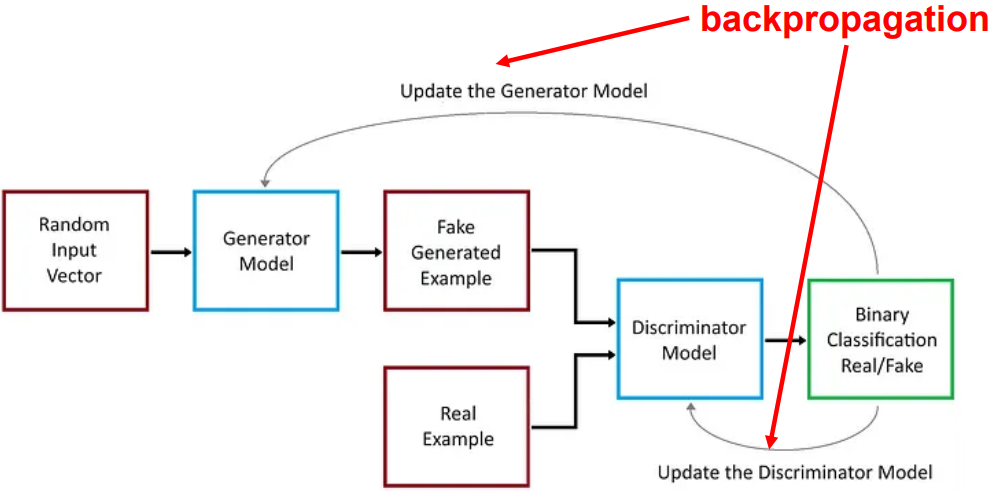
\includegraphics[width=0.8\textwidth]{img/backpropagation.png}
\end{figure}

\paragraph{Addestramento e Funzione di Costo}

Come illustrato nel diagramma di flusso, il generatore produce
un esempio falso che, insieme a un esempio reale, viene
sottoposto al discriminatore per una classificazione binaria
(Reale/Falso). Le due reti vengono addestrate in modo alternato,
non congiunto, attraverso un processo di backpropagation.
La funzione di costo (loss function) si ispira alla binary cross
entropy all'interno di un gioco minimax, dove il generatore
cerca di minimizzare la capacità del discriminatore di distinguere
i dati, mentre il discriminatore cerca di massimizzarla:

\[
    L_{GAN} = \min_G \max_D
    \mathbb{E}_{x \sim p_{data}(x)} [\log(D(x))]
    + \mathbb{E}_{z \sim p_z(z)} [\log(1 - D(G(z)))]
\]

\subsection{Adversarial Machine Learning e Attacchi}

Gli \textbf{Adversarial Examples (AE)} sono input per modelli
di machine learning che un attaccante ha intenzionalmente
progettato per indurre il modello a commettere un errore.
Gli AE rappresentano un aspetto significativo della sicurezza
dei sistemi basati sull'IA poiché costituiscono un problema
concreto nella sicurezza dell'IA (AI safety) che può essere
affrontato nel breve termine. Inoltre, risolvere il problema
degli AE è sufficientemente difficile da richiedere un serio
sforzo di ricerca.

Il principio di funzionamento è visibile nelle immagini
dimostrative: aggiungendo una perturbazione impercettibile
(rumore calcolato) all'immagine di un panda, il modello
classifica l'immagine risultante come ``gibbone'' con una
confidenza al 99.3\%. Analogamente, nel mondo fisico
l'applicazione di adesivi su un segnale di ``STOP'' può
ingannare un sistema di visione artificiale, facendogli
fallire il riconoscimento.

\begin{figure}[H]
    \centering
    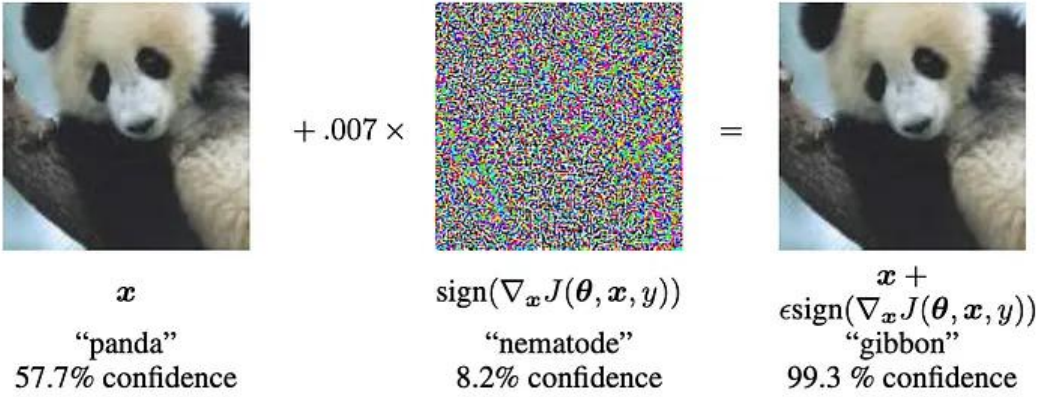
\includegraphics[width=0.8\textwidth]{img/AE.png}
\end{figure}

\subsubsection{Fast Gradient Sign Method (FGSM)}

\paragraph{Principio di Funzionamento}

Un metodo per creare esempi avversari consiste nel determinare
quanto ciascuna caratteristica (feature) contribuisca al valore
della funzione di costo (loss value) e aggiungere una
perturbazione di conseguenza. Questo approccio risulta rapido
perché è semplice calcolare il contributo di ogni input alla
loss utilizzando la regola della catena (chain rule) e trovando
i gradienti necessari.

\paragraph{Algoritmo FGSM}

Il \textbf{Fast Gradient Sign Method (FGSM)} opera calcolando il
gradiente della funzione di costo rispetto alla matrice di input,
mantenendo costanti i parametri del modello poiché questo non è
in fase di addestramento. L'unico obiettivo è ingannare il
modello già addestrato. Come mostrato nello schema logico, il
processo si articola in tre fasi: il calcolo del gradiente, la
generazione della perturbazione isolando il segno del gradiente
per una magnitudine $\epsilon$ e infine l'applicazione della
perturbazione all'input originale per creare l'esempio avversario.

\begin{figure}[H]
    \centering
    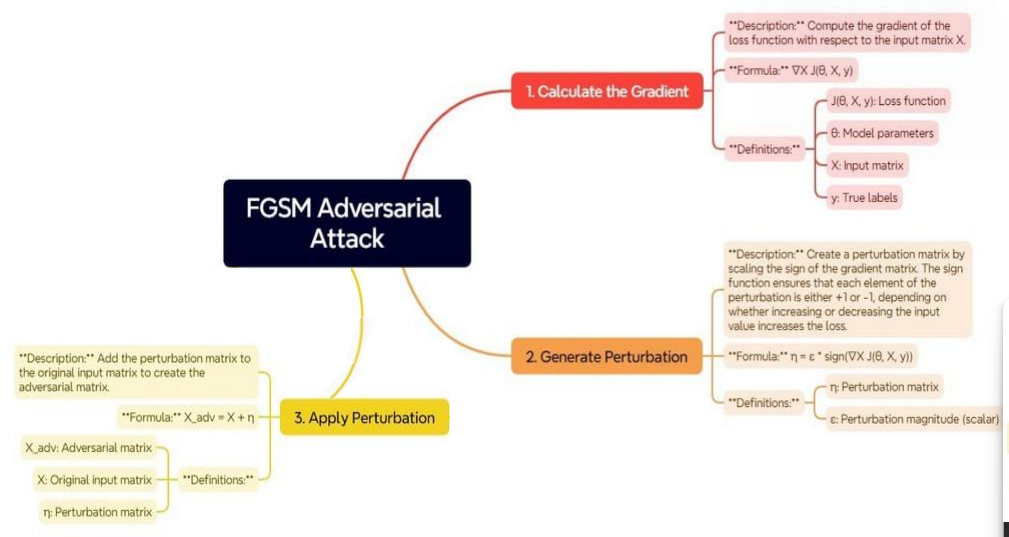
\includegraphics[width=1\textwidth]{img/FGSM.png}
\end{figure}

\paragraph{Formulazione Matematica}

Il metodo FGSM è uno dei più semplici e diffusi. Per un'istanza
di input, esso sfrutta i gradienti della perdita rispetto
all'input stesso per creare una nuova istanza che massimizzi
la perdita, ingannando così la rete. La formula che descrive
l'attacco è:
\[
    X_{adv} = X + \epsilon \cdot
    \text{sign}(\nabla_X J(\theta, X, y))
\]
dove $X$ è l'input originale, $\theta$ sono i parametri del
modello e $\epsilon$ è l'entità della perturbazione.

\paragraph{Interpretazione Grafica}

Osservando il grafico della funzione di costo, si nota la
differenza rispetto all'addestramento standard. Mentre durante
l'addestramento ci si muove nella direzione opposta al gradiente
per minimizzare la perdita (discesa del gradiente), nell'attacco
FGSM ci si muove nella direzione del gradiente per massimizzare
la perdita, spostando l'input verso una regione di
classificazione errata.

\begin{figure}[H]
    \centering
    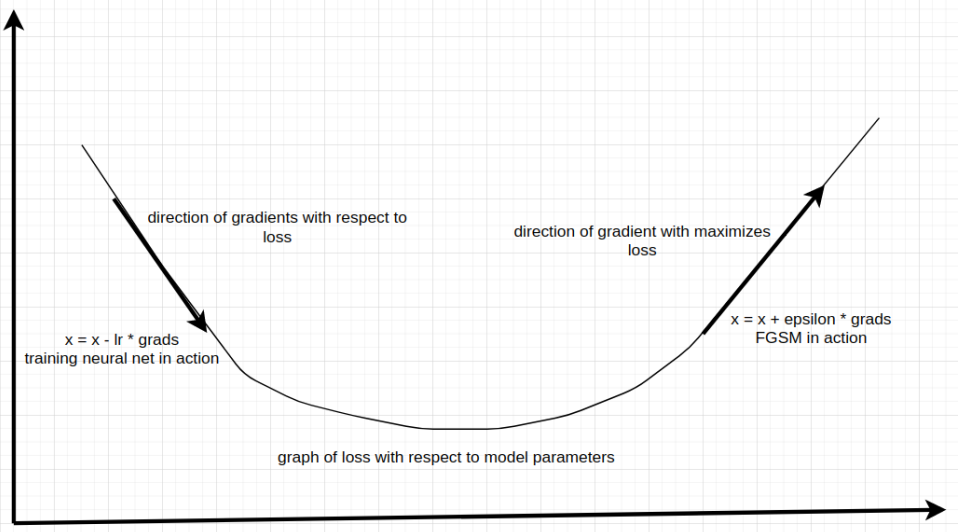
\includegraphics[width=0.8\textwidth]{img/gradientLoss.png}
\end{figure}

\paragraph{Sfide Specifiche nelle Reti}

Mentre l'utilizzo di questi approcci risulta piuttosto semplice
per le immagini, l'applicazione alla sicurezza è più complessa.
Nelle reti, non tutte le caratteristiche sono buoni candidati
per essere perturbate e sorge il problema di quanto perturbare
le caratteristiche candidate. Esiste un problema di scala: se
per le immagini la gestione è agevole, per il dataset di
networking è più insidiosa.

\paragraph{Risultati Sperimentali}

Analizzando i risultati dell'attacco FGSM sul dataset
CIC-IDS 2018, si osserva come l'efficacia del modello decada
all'aumentare della perturbazione. Una tabella mostra che con
una perturbazione dello 0\%, l'accuratezza è del 99.83\%, ma
crolla al 54.01\% con una perturbazione del 20\%, dimostrando
la vulnerabilità del modello standard. L'addestramento avversario
(Adversarial training) riesce a mantenere l'accuratezza sopra il
98\% anche sotto attacco.

\begin{figure}[H]
    \centering
    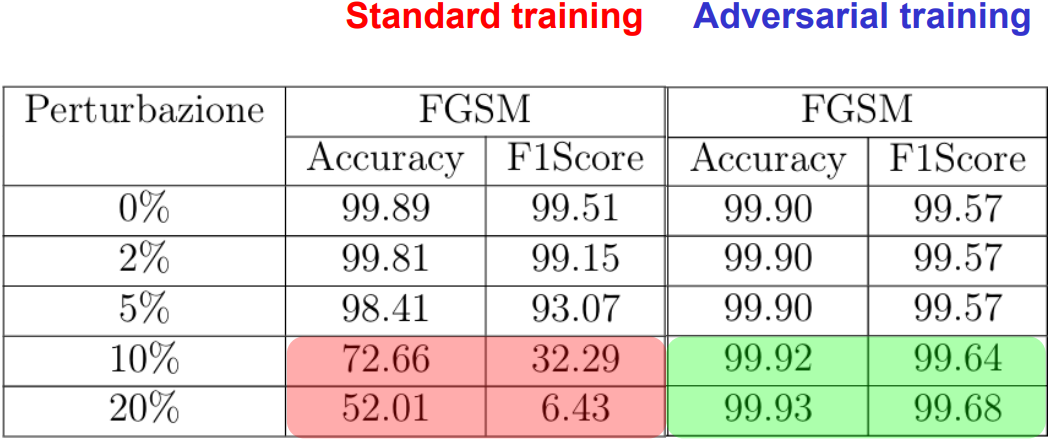
\includegraphics[width=0.8\textwidth]{img/dataset.png}
\end{figure}

\paragraph{Vantaggi del Metodo}

Il metodo FGSM presenta diversi vantaggi. In primo luogo, la sua
semplicità lo rende facile da comprendere e implementare.
Inoltre, dimostra un'elevata efficienza, poiché richiede solo un
passaggio in avanti (forward pass) e uno all'indietro (backward
pass) attraverso il modello. Infine, gode della proprietà di
``trasferibilità'', per cui gli esempi avversari generati su un
modello spesso riescono a ingannare anche altri modelli.

\paragraph{Svantaggi e Limitazioni}

Tra gli svantaggi, si segnala una robustezza limitata, in quanto
gli esempi creati con FGSM potrebbero non resistere a
trasformazioni diverse. È inoltre affetto da vulnerabilità nota
alle strategie di difesa, rendendo necessari metodi di
addestramento avversario più sofisticati. Infine, trattandosi di
un attacco white-box, richiede la conoscenza della rete neurale
artificiale per essere eseguito.

\subsubsection{Approfondimenti Tecnici e Varianti}

\paragraph{Requisiti White-Box}

Per applicare FGSM, è necessario disporre del modello completo
per calcolare il gradiente. In particolare, si richiede il
gradiente dei \textbf{LOGITS} di prima dell'applicazione della
funzione softmax. I logits permettono di preservare meglio il
comportamento del modello rappresentando la superficie di
separazione grezza prima della normalizzazione (punteggio di
confidenza che la rete assegna a ciascuna classe ma ancora
non normalizzata).

\paragraph{Importanza dei Logits}

Lavorare con i logits è preferibile poiché logits differenti
possono produrre le stesse probabilità se differiscono per una
costante, un'informazione che viene persa dopo la softmax.
Le differenze nei logits sono quindi più significative delle
differenze nelle probabilità, in quanto non soffrono degli
effetti di saturazione tipici della funzione softmax.

\paragraph{Approssimazione del Gradiente}

Qualora il gradiente non sia disponibile direttamente, è
possibile utilizzare approssimazioni tramite una funzione di
costo o direttamente sulla probabilità. Ad esempio, il gradiente
può essere stimato calcolando la differenza finita tra le
probabilità ottenute perturbando l'input leggermente in direzioni
opposte. In questo modo si può calcolare un vettore $X_{adv}$
approssimato.

\paragraph{Estensioni Iterative: PGD e HSJA}

Un'estensione naturale è il \textbf{Projected Gradient Descent
(PGD)}, che può essere visto come una versione iterativa di
FGSM e rappresenta lo stato dell'arte per l'addestramento
avversario. È un approccio white-box che richiede il calcolo del
gradiente o una sua approssimazione e non funziona con etichette
rigide (hard labels). Al contrario, l'\textbf{Hop Skip Jump
Attack (HSJA)} è un approccio black-box che funziona con hard
labels senza conoscenza della rete, stimando il gradiente tramite
campionamenti mirati, risultando computazionalmente efficiente.

\subsection{Attacchi Avanzati: PGD e HSJA}

\subsubsection{Projected Gradient Descent (PGD)}

\paragraph{Definizioni Fondamentali}

Per definire il PGD, partiamo da un input originale $x_0$
classificato correttamente e definiamo un budget di perturbazione
$\epsilon$, tipicamente con norma $L_\infty$. La dimensione del
passo $\alpha$ è solitamente impostata come frazione del budget
(es. $\epsilon/T$). Si definisce inoltre la proiezione
$\Pi_{B_{\epsilon}}(x_0)$ sulla ``bolla'' attorno al punto $x_0$
realizzata tramite una funzione di clip che mantiene i valori
entro l'intervallo $[x_0 - \epsilon, x_0 + \epsilon]$.

\paragraph{Obiettivo dell'Attacco}

L'obiettivo è partire da $x_0$ e trovare un esempio avversario
$x_{adv}$ tale che la classificazione risulti errata
($f(x_{adv}) \neq y_{true}$), pur mantenendo $x_{adv}$ e $x_0$
della stessa classe dal punto di vista visivo o semantico, ovvero
assicurandosi che la perturbazione sia contenuta entro i limiti
stabiliti.

\paragraph{Algoritmo Iterativo}

Il PGD opera attraverso un ciclo iterativo. Per ogni passo $t$
fino a $T-1$ si aggiorna l'input seguendo la direzione del segno
del gradiente (come in FGSM), ma proiettando immediatamente il
risultato all'interno del vincolo di perturbazione definito.
La formula di aggiornamento è:
\[
    x_{t+1} = \Pi_{B_{\epsilon}}(x_0)
    \left( x_t + \alpha \cdot
    \text{sign}(\nabla_x J(\theta, x_t, y)) \right)
\]

\paragraph{Condizioni di Arresto}

Il ciclo termina al raggiungimento del numero massimo di
iterazioni o al verificarsi delle condizioni di successo nel
trovare un campione avversario ($f(x_{t+1}) \neq y_{true}$),
o uno stallo nel processo (la differenza tra iterazioni scende
sotto una soglia $\eta$), o la saturazione della funzione di
costo.

\subsubsection{Hop Skip Jump Attack (HSJA)}

\paragraph{Individuazione Black-Box}

L'algoritmo HSJA lavora in modalità black-box con etichette
rigide. La fase di inizializzazione mira a trovare un primo
campione avversario $x_{adv}$ partendo da un campione pulito
$x_0$. Il processo prevede lo spostamento in direzioni casuali
(tramite un versore $u$) entro un budget definito fino a quando
non si individua un punto in cui la classificazione del modello
cambia rispetto a quella originale. Si ottiene così
$x^0_{adv} = x_0 + d \cdot v$ tale che
$f(x^0_{adv}) = f(x_0 + \delta_0 $u$)\neq f(x_0)$.

\paragraph{Fase di Hop}

Una volta trovato il punto avversario, l'algoritmo esegue la
fase di ``Hop'' verso il confine di separazione. Si calcola
$x_t^{bd}$ (boundary) tramite una ricerca binaria (Binary
Search) lungo la linea che collega il punto avversario corrente
$x_{adv}$ e l'originale $x_0$. Il punto di confine viene
identificato come il primo dove, per un piccolo spostamento,
la classificazione cambia.

\paragraph{Fase di Skip}

Successivamente, nella fase di ``Skip'', l'obiettivo è trovare
un vettore ortogonale alla superficie di separazione per muoversi
lungo di essa. Non conoscendo il modello, si stima il gradiente
della normale al confine calcolando la media su $m$ campioni
perturbati casualmente attorno al confine.

\paragraph{Fase di Jump}

La fase finale del ciclo è il ``Jump'' nella regione avversaria.
Si aggiorna il campione avversario spostandosi dal confine nella
direzione del gradiente stimato:
\[
    x_{adv}^{t+1} = x_t^{bd} + \xi_t
    \frac{g_t}{||g_t||_2}
\]
Il passo $\xi_t$ viene regolato dinamicamente: se il nuovo punto
non è avversario, il passo viene dimezzato fino a soddisfare la
condizione di misclassificazione.

\paragraph{Ciclicità del Processo}

Come illustrato nel diagramma geometrico, il processo
Hop-Skip-Jump viene ripetuto in un ciclo. L'obiettivo finale è
trovare un campione avversario che sia il più vicino possibile
al campione di riferimento pulito, raffinando progressivamente
la perturbazione.

\begin{figure}[H]
    \centering
    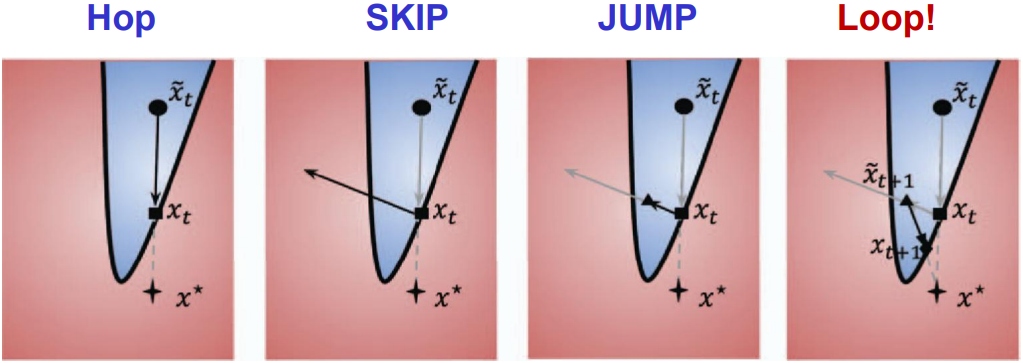
\includegraphics[width=0.8\textwidth]{img/hsja.png}
\end{figure}

\paragraph{Difficoltà di Difesa}

Concludendo sugli esempi avversari, è importante sottolineare
che è difficile difendersi contro di essi per due motivi
principali: in primo luogo, è arduo costruire un modello teorico
del processo di creazione degli esempi avversari; in secondo
luogo, la difesa richiede che i modelli diano il risultato
corretto per ogni possibile input. I modelli attuali funzionano
molto bene, ma solo in una frazione molto piccola di tutti i
possibili input che potrebbero incontrare, lasciando spazio
a vulnerabilità.

\subsection{Reinforcement Learning (RL)}

\subsubsection{Fondamenti e Ciclo di Apprendimento}

Passiamo ora al \textbf{Reinforcement Learning (RL)}, una
tecnica di machine learning che permette a un agente di
apprendere in un ambiente interattivo per tentativi ed errori
(trial and error) utilizzando il feedback delle proprie azioni
ed esperienze. L'RL utilizza ricompense e punizioni come segnali
per rinforzare comportamenti positivi o negativi.

\begin{figure}[H]
    \centering
    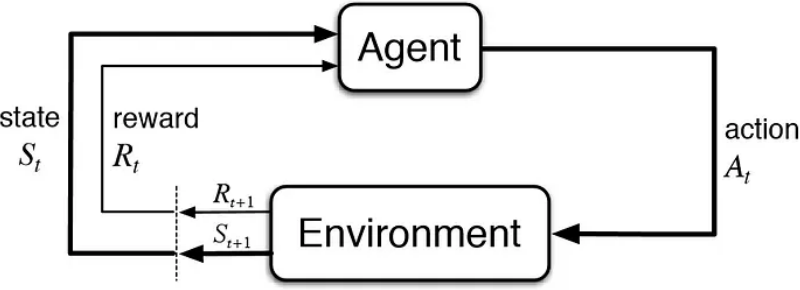
\includegraphics[width=0.7\textwidth]{img/rl.png}
\end{figure}

\paragraph{Elementi Principali}

Il ciclo di apprendimento, coinvolge
l'interazione continua tra Agente e Ambiente attraverso stati,
azioni e ricompense. Gli elementi costitutivi sono: l'
\textbf{Ambiente}, ovvero il mondo fisico in cui l'agente opera;
lo \textbf{Stato}, che descrive la situazione corrente; la
\textbf{Ricompensa (Reward)}, che è il feedback dell'ambiente;
la \textbf{Politica (Policy)}, il metodo che mappa lo stato alle
azioni; e il \textbf{Valore}, che rappresenta la ricompensa
futura attesa.

\paragraph{Fondamenti Tecnici}

I \textbf{Processi Decisionali di Markov (Markov Decision
Processes)} forniscono le basi teoriche per l'RL. Questa tecnica
entra in azione in ambienti del mondo reale, dove spesso manca
una conoscenza a priori delle dinamiche dell'ambiente stesso.

\subsubsection{Applicazioni al Networking}

\paragraph{Limiti del Paradigma Classico}

Nel paradigma classico di progettazione delle reti, il
progettista assume un modello semplificato del sistema, specifica
obiettivi di alto livello e sviluppa un algoritmo ad hoc per
risolvere il problema. Tuttavia, poiché le reti e le applicazioni
sono cresciute in complessità ed eterogeneità, progettare
algoritmi fissi che funzionino bene in una varietà di condizioni
è diventato estremamente difficile. Gli approcci classici spesso
sacrificano le prestazioni in favore dell'universalità,
costringendo i progettisti a sviluppare soluzioni puntuali ed
euristiche specializzate per ogni ambiente.

\paragraph{Obiettivo dell'RL nelle Reti}

L'obiettivo dell'applicazione dell'RL è sviluppare sistemi in
grado di imparare a ottimizzare le prestazioni autonomamente.
In questo nuovo scenario, il progettista architetta un framework
per la raccolta dei dati, la sperimentazione e l'apprendimento,
ed è il sistema stesso a scoprire automaticamente le azioni di
basso livello necessarie per raggiungere gli obiettivi di
gestione delle risorse di alto livello. Esempi applicativi
includono protocolli di controllo sensibili al contesto per lo
streaming video adattivo e schedulatori (schedulers) per carichi
di lavoro complessi e su larga scala.


